\documentclass[conference]{IEEEtran}
\IEEEoverridecommandlockouts
% The preceding line is only needed to identify funding in the first footnote. If that is unneeded, please comment it out.
\usepackage{cite}
\usepackage{amsmath,amssymb,amsfonts}
\usepackage{algorithmic}
\usepackage{textcomp}
\usepackage{xcolor}
\usepackage{url}
\usepackage{graphicx}
\graphicspath{ {./images/} }
\def\BibTeX{{\rm B\kern-.05em{\sc i\kern-.025em b}\kern-.08em
    T\kern-.1667em\lower.7ex\hbox{E}\kern-.125emX}}
\begin{document}

\title{Assignment report for the course\\ Automated Planning: Theory and Practice\\
{\footnotesize Master's degree in Artificial Intelligence Systems;
A.Y 2022/2023;
Marco Roveri}
}

\author{\IEEEauthorblockN{Joy Battocchio}

\and
\IEEEauthorblockN{Davide Guidolin}

% \IEEEauthorblockA{\textit{dept. name of organization (of Aff.)} \\
% \textit{name of organization (of Aff.)}\\
% City, Country \\
% email address or ORCID}
}

\maketitle

\section{Introduction}
The following report aims to give a detailed explanation of the solutions of the 5 problems proposed in the assignment.
The problems considered a scenario where one or more robots have to deliver emergency supplies to injured people located in space.
These were the initial explicit assumptions:
\begin{itemize}
    \item Each injured person is at a specific location, and does not move.
    \item Each box is initially at a specific location and can be filled with a specific content if empty. Box contents shall be modeled in a generic way, so that new contents can easily be introduced in the problem instance.
    \item Each person either has or does not have a box with a specific content.
    \item There can be more than one person at any given location.
    \item The robotic agents can move directly between arbitrary locations.
    \item We want to be able to expand this domain for multiple robotic agents in the future.
\end{itemize}  
While the suggested actions were the following:
\begin{itemize}
    \item Fill a box with a content. Robot box and content must be in the same place, box must be empty.
    \item Empty a box, satisfying the person at that specific location.
    \item Pick up a box located in the same place as the robot.
    \item Move to another location.
    \item Deliver a box.
\end{itemize}

Based on these assumptions here is the formulated solution used in all problems.
We considered 5 main types:
\begin{itemize}
    \item Robot
    \item Person
    \item Location
    \item Box
    \item Content
\end{itemize}
and 5 main actions:
\begin{itemize}
    \item Fill 
    \item Empty
    \item Load
    \item Move
    \item Unload
\end{itemize}

The main workflow the robot follow to satify a person is to \textbf{fill} a box with a content,
\textbf{load} the box on itself and \textbf{move} carrying the box toward the destination.
Once it gets where the person is located it \textbf{unloads} the box and \textbf{empties} it giving the content to the person.
After that the robot needs to restart in order to satisfy another person, so it can re-use the same box as before and carry it to the place where the supplies are stored, or look for another box.
We assume the supplies are infinite where stored, but only one portion can fit in a box, so if 2 people need the same supply the robot must re-fill with it.
\\
For doing so the folllowing informations are needed:
\begin{itemize}
    \item Where a robot is (\textbf{robot-at}).
    \item If a robot is carrying a box(\textbf{robot-loaded}).
    \item Which box a robot is carrying (\textbf{robot-has}).
    \item If a box is full (\textbf{box-full}).
    \item Where a box is (\textbf{box-at}).
    \item What is the content of a box (\textbf{box-contains}).
    \item Where a supply is stored (\textbf{content-at}); specified in the initial assumptions of the problem and fixed.
    \item Where a person is (\textbf{person-at}); specified in the initial assumptions of the problem and fixed.
    \item What supply a person has (\textbf{person-has}); which represent the goal.
\end{itemize}
For all problems we used \textbf{negative preconditions} since the predicates make more sense this way and it is supported by almost every planner.
We also made a version without \textbf{negative precondition} that has very few differences, it is sufficient to use \textbf{box-empty} and \textbf{robot-unloaded} and remove the negated preconditions from the \textbf{move} action. 
Notice that this configuration ensure there are no constraints on the number of robots or boxes in order to satisfy any number of people.
\section{Problem 1}
The first problem was solved simply by implementing what is described in the introduction above.
We set the environment with 1 robot, 3 people, 5 locations (one of which is the depot where the supplies are stored), 2 boxes and 3 types of supply.
Initially the 3 people are scattered over the locations, while robot, boxes and supplies are in the depot.
The goal is to deliver medicine to person2, and to deliver food and medicine to person3; person1 does not need anything.

\section{Problem 2}
The second problem required to think about the \textbf{move} action in a different persective, 
ensuring that a robot can load the boxes on a carrier instead of itself, and that the carrier can be transported by a robot to the destinations.\\
The solution we developed are two, the first one is simpler since it only has an additional type \textbf{carrier} and its \textbf{capacity} is represented through a function.
The initial capacity of each carrier can be specified in the problem, and it is managed through the usage of fluents: \textbf{load} can be performed only if the capacity is greater than 0, and the effect is to decrement it, the opposite for \textbf{unload}.\\
Another solution has been implemented since the first one relies on the \textbf{fluents} requirement, which is not supported by many planner we used.
We took inspiration by an example provided during the lab session, in which each a new type called \textbf{capacity-number} is used to described all the possible capacities.
Then for each \textbf{load} and \textbf{unload} operation done on the carrier is important not to forget to specify the precondition \textbf{capacity-predecessor} through which we ensure the numbers we use to upload the capacity are consequent.
The order of the capacity is specified in the problem as follows:
\begin{verbatim}
(capacity_predecessor capacity_0 capacity_1)
(capacity_predecessor capacity_1 capacity_2)
(capacity_predecessor capacity_2 capacity_3)
(capacity_predecessor capacity_3 capacity_4)
\end{verbatim}
Plus the initial capacity of each carrier (4 as requested):
\begin{verbatim}
    (capacity carrier1 capacity_4)
\end{verbatim}
Finally the last modification with respect to the first problem is the \textbf{move} action, which no longer allow a robot to carry a box, but a carrier instead.
Thanks to this any robot can carry any carrier, even if loaded by another robot.\\
To test it with a more complex environment we increased the number of people to 6, the boxes to 5, the locations to 8 and the supplies to 5, the robot and the carrier are just one each, as requested in the assignement.
Of course there are no constraints neither in the number of robots nor of carriers.
From this point on, all next problems are solved using solution 2 described above as base.
\section{Problem 3}
Problem number 3 required a hierarchical implementation of the actions.
We decided to construct it as described in the diagram \ref{Actions diagram}
The main task is to \textbf{satisfy} a person delivering to him/her a specific supply.
To do that the robot first has to \textbf{get the content}, then to \textbf{delivery} it.
To \textbf{get the content} the robot \textbf{gets to} the place where the supply is stored, and \textbf{loads} it on the carrier (\textbf{fill} + \textbf{load}).
The \textbf{delivery} consists of \textbf{get to} the place where the person is and \textbf{unload the content} (\textbf{unload} + \textbf{empty}).
This is a standard workflow, of which there are some variations listed here:
\begin{itemize}
    \item A robot could already have the needed supply in a box it is carrying. For this we have an alternative method for the \textbf{get\_content} task, which is \textbf{m\_already\_got\_content} that is implemented by the action \textbf{no\_load}, which basically does nothing.
    \item A robot could already be where it has to go, so the \textbf{get\_to} task is also implemented using the \textbf{m\_already\_there} method that calls the \textbf{no\_move} action.
    \item In case the number of boxes is less than the number of people to satisfy, A robot must keep the box after delivering the supplies, to do that there are 2 implementations for the \textbf{delivery} action, one that \textbf{load} the box on the carrier after it empties it and one that does not.
    \item When a robot wants to re-use a box, it needs to \textbf{get\_content} using a box it is already in the carrier, for this reason there are 2 implementations of the \textbf{get\_content} task, one \textbf{unload} a box from the carrier before filling it and load it, the other does not.
\end{itemize} 
To test it we kept the same environment as in problem 2, with 7 \textbf{satisfy} tasks to perform.
We had to specify an ordering to keep the searching space sufficiently small and to find a plan in little time, if no temporal constraints are put, the ordering can be removed.

The problem definition is reported in \textit{Fig. \ref{problem3_problem}} while the obtained plan is reported in \textit{Fig. \ref{problem3_plan}}.
\section{Problem 4}
For solving problem 4 we were asked to use durative actions.
The chosen duration are the following:
\begin{itemize}
    \item Fill: 5
    \item Load: 4
    \item Move: 10
    \item Unload: 2
    \item Empty: 3
\end{itemize}
We considered the robots to have one arm, this means it cannot load several boxes at the same time, or loading and filling as well as unloading and emptying at the same time.\\
The only case possible where a robot could make two actions in parallel are if it starts unloading a box from the carrier while still moving.
To manage the possibility and not possibility to parallelize actions the predicates \textbf{busy} has been added.
It refers to a robot and is used to understand when the successive action can begin.
In fact all the non-parallel actions have the same effects:
\begin{verbatim}
and     (at start (busy ?r))
        (at end (not (busy ?r))
        ...
\end{verbatim}
and the same precondition:
\begin{verbatim}
and     (at start (not(busy ?r)))
        ...
\end{verbatim}
The actions \textbf{empty}, \textbf{fill} and \textbf{load} have as precondition $(over all (robot-at ?r ?x))$
meaning that for all the execution of that action the robot must be at that location. \\
The \textbf{unload} action instead has as precondition $(at end(robot-at ?r ?x))$ which means that we only need to be at the right location
when the box touches the ground, so when the action \textbf{unload} ends.
\section{Problem 5}
For solving problem 5 we were asked to implement problem 4 using PlanSys2 \cite{plansys2} that is a software platform used to create, execute and monitor plans on a robotic agent. We used PlanSys2 inside the 
Robot Operating System 2 (ROS2) \cite{ros2}.

To implement the problem in PlanSys2 we started from a simple example \footnote{\url{https://github.com/PlanSys2/ros2_planning_system_examples/tree/master/plansys2_simple_example}} and we modified the necessary files that are:
\begin{itemize}
    \item \verb+launch/launcher.py+ \\ 
    that contains the code to select the domain and run the executables that implement the PDDL actions. Here we only changed the names of the actions and the project name.
    \item \verb+CMakeLists.txt+ and \verb+package.xml+ \\
    in which we only had to change the project name
    \item \verb+launch/commands+ \\
    that contains the definition of the problem
    \item \verb+pddl/domain.pddl+ \\
    that contains the pddl domain
    \item all the files in \verb+src/+ \\
    that contain the implementation of the actions
\end{itemize}

Since we didn't have a real robot, we used fake actions that simulate the 
behaviour of a robot by waiting for an appropriate amount of time before ending the action and by logging what the robot should do.

PlanSys2 supports two planners: TFD \cite{tfd} and POPF \cite{popf}.
We tried both the planners because POPF was slow in finding the plan and it 
was stopped early inside the \verb+plansys2_terminal+ while TFD was able to find the plan faster but, since it isn't the default planner in PlanSys2 it required more work for the setup. Moreover POPF does not support the \verb+negative-preconditions+ requirement so the domain was slightly different from the one used in TFD.

Regarding the TFD setup we had to modify the source code because PlanSys2 was not able to find the correct TFD path, however everything is explained in the Github repository \footnote{\url{https://github.com/Davide-Guidolin/Automated-Planning-Project}}.

The problem definition is reported in \textit{Fig. \ref{problem5_problem}}, the obtained plan using POPF is reported in \textit{Fig. \ref{problem5_plan_popf}} while the obtained plan using TFD is reported in \textit{Fig. \ref{problem5_plan_tfd}}.
\section{Final comment}
The main workflow to solve all the problems was the following: 
\begin{itemize}
    \item Understand the assignment text, including environment constraints and goals.
    \item Formulate an idea of the environment as general as possible, in order to include also all the sub-cases.
    \item Write the PDDL domain and problem files with a goal that should be achieved by few actions.
    \item Enlarge the goal with a bottom-up approach to finally reach the final goal, solving the issues encountered at each step. 
\end{itemize}
Following this simple steps we managed to solve all the problems in little time.
A big issue that has been encountered and delayed the work was finding the correct planner and set everything correctly: 
we found that many planners don't support simple requirements such as "fluents" or "negative-precondition", so we had to try many and to develop different
solutions in order to finally choose not only the best one, but the one with less compatibility problems.\\
This is the case of problem 2 and problem 5, where two different solutions are proposed for each one.
Problem 5 was in particular the most problematic since the deafult planner do not support negative preconditions, and we took a while to find out this was the issue that made it not work,
since the informations given by the planner concerning the errors are never exhaustive.\\
An interesting observation is that if no optimization is requested, different planners may take very different path to reach the goal, sometimes the difference is of several actions.
This can be noticed especially when dealing with those problems implying the capacity of the carrier, and so the possibility to carry many boxes at the same time.
The heuristic of some planners, in fact, made them repeat the \textbf{load} action many times in a row exploiting the full capacity of the carrier and resulting in less trips of the robot,
whereas others prefered to move as soon as possible to the satisfaction of every single goal resulting in more trips and a less efficient plan.
We recognize this is not a real issue since no optimization was requested, but it's worth to notice that in a general search case heuristics can make a big difference.
Another big difference found among different planners that can be attributed to the heuristics is the search time needed to find a plan.\\
It could be interesting to evaluate the performances of different planners requesting an optimization in the plan.
\bibliographystyle{ieeetr}
\bibliography{mybib}
\pagebreak
\onecolumn

\section{Appendix}
\begin{figure}[h!]
    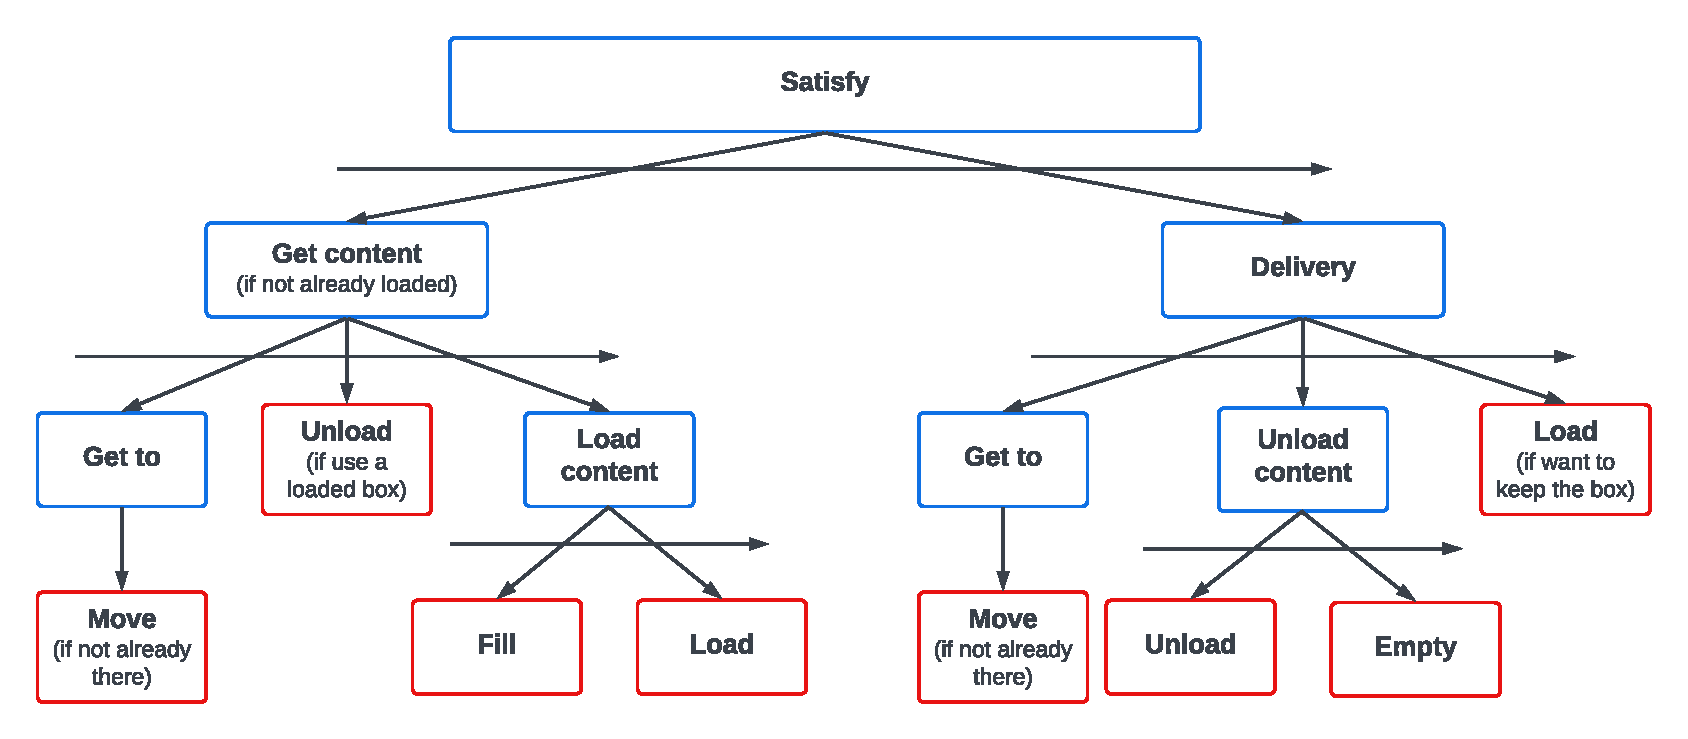
\includegraphics[scale = 0.66]{images/Actions_diagram.pdf}
    \caption{Hierarchical tasks diagram}
    \label{Actions diagram}
\end{figure}

\begin{figure}[h!]
    \begin{verbatim}
    (define (problem robo-doctor_1) (:domain robo-doctor_1)
    (:objects 
        robot1                                  - robot
        person1 person2 person3                 - person
        depot loc1 loc2 loc3 loc4               - location
        box1 box2                               - box
        medicine food tool                      - content
    )

    (:init
        (person-at person1 loc1)
        (person-at person2 loc3)
        (person-at person3 loc4)
        (robot-at robot1 depot)
        (box-at box1 depot)
        (box-at box2 depot)
        (content-at medicine depot)
        (content-at food depot)
        (content-at tool depot)
    )

    (:goal (and
        (person-has person2 medicine)
        (person-has person3 food)
        (person-has person3 medicine)
    ))
    )

    \end{verbatim}
    \caption{Problem 1}
    \label{problem1_problem}
\end{figure}

\begin{figure}[h!]
    \begin{verbatim}
        fill robot1 box1 food depot (1)
        load robot1 depot box1 (1)
        fill robot1 box2 medicine depot (1)
        move robot1 depot loc3 (1)
        move robot1 loc3 loc4 (1)
        unload robot1 loc4 box1 (1)
        empty robot1 loc4 box1 food person3 (1)
        move robot1 loc4 depot (1)
        load robot1 depot box2 (1)
        move robot1 depot loc3 (1)
        unload robot1 loc3 box2 (1)
        empty robot1 loc3 box2 medicine person2 (1)
        move robot1 loc3 loc4 (1)
        load robot1 loc4 box1 (1)
        move robot1 loc4 depot (1)
        unload robot1 depot box1 (1)
        fill robot1 box1 medicine depot (1)
        load robot1 depot box1 (1)
        move robot1 depot loc4 (1)
        unload robot1 loc4 box1 (1)
        empty robot1 loc4 box1 medicine person3 (1)
    \end{verbatim}
    \caption{Plan for problem 1}
    \label{problem1_plan}
\end{figure}

\begin{figure}[h!]
    \begin{verbatim}
        (define (problem robo-doctor_2) (:domain robo-doctor_2)
        (:objects 
            robot1                                              - robot
            person1 person2 person3 person4 person5 person6     - person
            depot loc1 loc2 loc3 loc4 loc5 loc6 loc7            - location
            box1 box2 box3 box4 box                             - box
            xanax bendage banana pizza hammer                   - content
            carrier1                                            - carrier
            capacity_0                                          - capacity_number
            capacity_1                                          - capacity_number
            capacity_2                                          - capacity_number
            capacity_3                                          - capacity_number
            capacity_4                                          - capacity_number
        )
        
        (:init
            (capacity carrier1 capacity_4)
            (person-at person1 loc1)
            (person-at person2 loc3)
            (person-at person3 loc4)
            (person-at person4 loc7)
            (person-at person5 loc2)
            (person-at person6 loc6)
            (carrier-at carrier1 depot)
            (robot-at robot1 depot)
            (box-at box1 depot)
            (box-at box2 depot)
            (box-at box3 depot)
            (box-at box4 depot)
            (content-at xanax depot)
            (content-at bendage depot)
            (content-at banana depot)
            (content-at pizza depot)
            (content-at hammer depot)
            (capacity_predecessor capacity_0 capacity_1)
            (capacity_predecessor capacity_1 capacity_2)
            (capacity_predecessor capacity_2 capacity_3)
            (capacity_predecessor capacity_3 capacity_4)
            )
        
        (:goal (and
            (person-has person1 hammer)
            (person-has person2 banana)
            (person-has person3 xanax)
            (person-has person3 hammer)
            (person-has person5 bendage)
            (person-has person6 bendage)
            (person-has person6 pizza)
            (person-has person6 xanax)
        ))
        )
        

    \end{verbatim}
    \caption{Problem 2}
    \label{problem2_problem}
\end{figure}

\begin{figure}
    \small
    \begin{verbatim}
        fill robot1 box1 banana depot (1)
        load robot1 depot box1 carrier1 capacity_3 capacity_4 (1)
        move robot1 carrier1 depot loc3 (1)
        unload robot1 loc3 box1 carrier1 capacity_3 capacity_4 (1)
        move robot1 carrier1 loc3 depot (1)
        load robot1 depot box2 carrier1 capacity_3 capacity_4 (1)
        move robot1 carrier1 depot loc3 (1)
        empty robot1 loc3 box1 banana person2 (1)
        move robot1 carrier1 loc3 depot (1)
        unload robot1 depot box2 carrier1 capacity_3 capacity_4 (1)
        fill robot1 box2 bendage depot (1)
        load robot1 depot box2 carrier1 capacity_3 capacity_4 (1)
        move robot1 carrier1 depot loc2 (1)
        unload robot1 loc2 box2 carrier1 capacity_3 capacity_4 (1)
        empty robot1 loc2 box2 bendage person5 (1)
        move robot1 carrier1 loc2 depot (1)
        fill robot1 box3 bendage depot (1)
        load robot1 depot box3 carrier1 capacity_3 capacity_4 (1)
        move robot1 carrier1 depot loc6 (1)
        unload robot1 loc6 box3 carrier1 capacity_3 capacity_4 (1)
        empty robot1 loc6 box3 bendage person6 (1)
        load robot1 loc6 box3 carrier1 capacity_3 capacity_4 (1)
        move robot1 carrier1 loc6 depot (1)
        unload robot1 depot box3 carrier1 capacity_3 capacity_4 (1)
        fill robot1 box3 hammer depot (1)
        load robot1 depot box3 carrier1 capacity_3 capacity_4 (1)
        move robot1 carrier1 depot loc1 (1)
        unload robot1 loc1 box3 carrier1 capacity_3 capacity_4 (1)
        move robot1 carrier1 loc1 depot (1)
        load robot1 depot box4 carrier1 capacity_3 capacity_4 (1)
        move robot1 carrier1 depot loc4 (1)
        unload robot1 loc4 box4 carrier1 capacity_3 capacity_4 (1)
        move robot1 carrier1 loc4 loc1 (1)
        empty robot1 loc1 box3 hammer person1 (1)
        load robot1 loc1 box3 carrier1 capacity_3 capacity_4 (1)
        move robot1 carrier1 loc1 depot (1)
        unload robot1 depot box3 carrier1 capacity_3 capacity_4 (1)
        fill robot1 box3 pizza depot (1)
        load robot1 depot box3 carrier1 capacity_3 capacity_4 (1)
        move robot1 carrier1 depot loc4 (1)
        load robot1 loc4 box4 carrier1 capacity_2 capacity_3 (1)
        move robot1 carrier1 loc4 loc6 (1)
        unload robot1 loc6 box3 carrier1 capacity_2 capacity_3 (1)
        empty robot1 loc6 box3 pizza person6 (1)
        move robot1 carrier1 loc6 depot (1)
        unload robot1 depot box4 carrier1 capacity_3 capacity_4 (1)
        fill robot1 box4 hammer depot (1)
        load robot1 depot box4 carrier1 capacity_3 capacity_4 (1)
        move robot1 carrier1 depot loc4 (1)
        unload robot1 loc4 box4 carrier1 capacity_3 capacity_4 (1)
        empty robot1 loc4 box4 hammer person3 (1)
        load robot1 loc4 box4 carrier1 capacity_3 capacity_4 (1)
        move robot1 carrier1 loc4 depot (1)
        unload robot1 depot box4 carrier1 capacity_3 capacity_4 (1)
        fill robot1 box4 xanax depot (1)
        load robot1 depot box4 carrier1 capacity_3 capacity_4 (1)
        move robot1 carrier1 depot loc4 (1)
        unload robot1 loc4 box4 carrier1 capacity_3 capacity_4 (1)
        empty robot1 loc4 box4 xanax person3 (1)
        move robot1 carrier1 loc4 loc6 (1)
        load robot1 loc6 box3 carrier1 capacity_3 capacity_4 (1)
        move robot1 carrier1 loc6 depot (1)
        unload robot1 depot box3 carrier1 capacity_3 capacity_4 (1)
        fill robot1 box3 xanax depot (1)
        load robot1 depot box3 carrier1 capacity_3 capacity_4 (1)
        move robot1 carrier1 depot loc6 (1)
        unload robot1 loc6 box3 carrier1 capacity_3 capacity_4 (1)
        empty robot1 loc6 box3 xanax person6 (1)
    \end{verbatim}
    \caption{Plan for problem 2}
    \label{problem2_plan}
\end{figure}

\begin{figure}
    \begin{verbatim}
        (define (problem robo-doctor_2) (:domain robo-doctor_2)
        (:objects 
            robot1                                              - robot
            person1 person2 person3 person4 person5 person6     - person
            depot loc1 loc2 loc3 loc4 loc5 loc6 loc7            - location
            box1 box2 box3 box4                                 - box
            xanax bendage banana pizza hammer                   - content
            carrier1                                            - carrier
        )

        (:init
            (= (capacity carrier1) 4)
            (person-at person1 loc1)
            (person-at person2 loc3)
            (person-at person3 loc4)
            (person-at person4 loc7)
            (person-at person5 loc2)
            (person-at person6 loc6)
            (carrier-at carrier1 depot)
            (robot-at robot1 depot)
            (box-at box1 depot)
            (box-at box2 depot)
            (box-at box3 depot)
            (box-at box4 depot)
            (content-at xanax depot)
            (content-at bendage depot)
            (content-at banana depot)
            (content-at pizza depot)
            (content-at hammer depot)
            )

        (:goal (and
            (person-has person1 hammer)
            (person-has person2 banana)
            (person-has person3 xanax)
            (person-has person3 hammer)
            (person-has person5 bendage)
            (person-has person6 bendage)
            (person-has person6 pizza)
            (person-has person6 xanax)
        ))
        )
    \end{verbatim}
    \caption{Problem 2 using fluents}
    \label{problem2_problem_fluents}
\end{figure}

\begin{figure}[htp]
    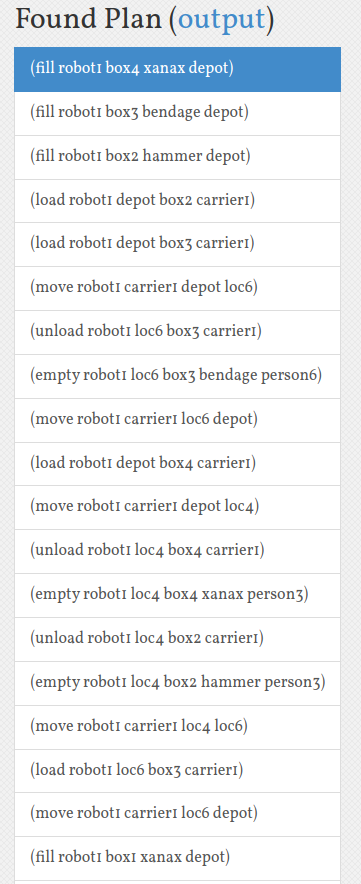
\includegraphics[scale = 0.66]{images/p2_fluents1.png}
    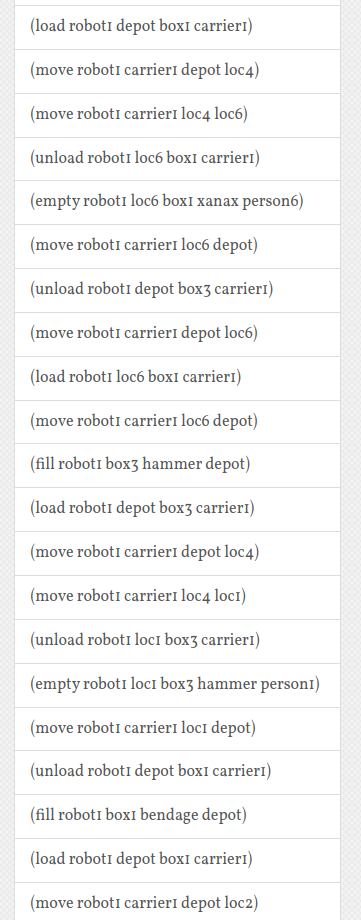
\includegraphics[scale = 0.66]{images/p2_fluents2.png}
    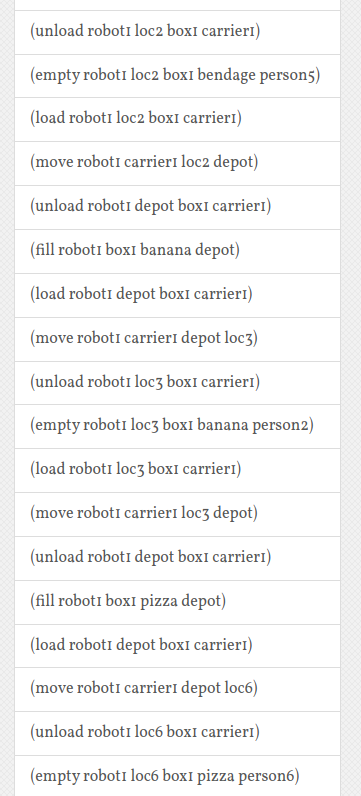
\includegraphics[scale = 0.66]{images/p2_fluents3.png}
    \caption{Plan for problem 2 using fluents}
    \label{problem2_plan_fluents}
\end{figure}

\begin{figure}[h!]
    \small
    \begin{verbatim}
        (define (problem robo-doctor_3) (:domain robo-doctor_3)
        (:objects 
            robot1                                              - robot
            person1 person2 person3 person4 person5 person6     - person
            depot loc1 loc2 loc3 loc4 loc5 loc6 loc7            - location
            box1 box2 box3 box4 box5                            - box
            xanax bendage banana pizza hammer                   - content
            carrier1                                            - carrier
            capacity_0                                          - capacity_number
            capacity_1                                          - capacity_number
            capacity_2                                          - capacity_number
            capacity_3                                          - capacity_number
            capacity_4                                          - capacity_number
            ; capacity_5                                          - capacity_number
        )

        (:htn
                :parameters ()
                :subtasks (and
                (task1 (satisfy person2 banana))
                (task2 (satisfy person3 xanax))
                (task3 (satisfy person3 hammer))
                (task4 (satisfy person5 bendage))
                (task5 (satisfy person6 bendage))
                (task6 (satisfy person6 pizza))
                (task7 (satisfy person6 xanax))    
                )
                :ordering (and
                (task1 < task2)
                (task2 < task3)
                (task3 < task4)
                (task4 < task5)
                (task5 < task6)
                (task6 < task7)
                )
            )
        (:init
            (capacity carrier1 capacity_4)
            (person-at person1 loc1)
            (person-at person2 loc3)
            (person-at person3 loc4)
            (person-at person4 loc7)
            (person-at person5 loc2)
            (person-at person6 loc6)
            (carrier-at carrier1 depot)
            (robot-at robot1 depot)
            (box-at box1 depot)
            (box-at box2 depot)
            (box-at box3 depot)
            (box-at box4 depot)
            (box-at box5 depot)
            (content-at xanax depot)
            (content-at bendage depot)
            (content-at banana depot)
            (content-at pizza depot)
            (content-at hammer depot)
            (capacity_predecessor capacity_0 capacity_1)
            (capacity_predecessor capacity_1 capacity_2)
            (capacity_predecessor capacity_2 capacity_3)
            (capacity_predecessor capacity_3 capacity_4)
            )
        )
    \end{verbatim}
    \caption{Problem 3}
    \label{problem3_problem}
\end{figure}

\begin{figure}
    \footnotesize
    \begin{verbatim}
        0: SHOP_methodm_satisfy_0_precondition(person2,banana)
        1: SHOP_methodm_get_content_nobox_1_precondition(banana,depot)
        2: no_move(robot1,carrier1,depot)
        3: fill(robot1,box2,banana,depot)
        4: load(robot1,depot,box2,carrier1,capacity_3,capacity_4)
        5: SHOP_methodm_delivery_wbox_4_precondition(person2,loc3)
        6: move(robot1,carrier1,depot,loc3)
        7: unload(robot1,loc3,box2,carrier1,capacity_3,capacity_4)
        8: empty(robot1,loc3,box2,banana,person2)
        9: load(robot1,loc3,box2,carrier1,capacity_3,capacity_4)
        10: SHOP_methodm_satisfy_0_precondition(person3,xanax)
        11: SHOP_methodm_get_content_nobox_1_precondition(xanax,depot)
        12: move(robot1,carrier1,loc3,depot)
        13: fill(robot1,box4,xanax,depot)
        14: load(robot1,depot,box4,carrier1,capacity_2,capacity_3)
        15: SHOP_methodm_delivery_nobox_3_precondition(person3,loc4)
        16: move(robot1,carrier1,depot,loc4)
        17: unload(robot1,loc4,box4,carrier1,capacity_2,capacity_3)
        18: empty(robot1,loc4,box4,xanax,person3)
        19: SHOP_methodm_satisfy_0_precondition(person3,hammer)
        20: SHOP_methodm_get_content_wbox_2_precondition(hammer,depot)
        21: move(robot1,carrier1,loc4,depot)
        22: unload(robot1,depot,box2,carrier1,capacity_3,capacity_4)
        23: fill(robot1,box2,hammer,depot)
        24: load(robot1,depot,box2,carrier1,capacity_3,capacity_4)
        25: SHOP_methodm_delivery_wbox_4_precondition(person3,loc4)
        26: move(robot1,carrier1,depot,loc4)
        27: unload(robot1,loc4,box2,carrier1,capacity_3,capacity_4)
        28: empty(robot1,loc4,box2,hammer,person3)
        29: load(robot1,loc4,box2,carrier1,capacity_3,capacity_4)
        30: SHOP_methodm_satisfy_0_precondition(person5,bendage)
        31: SHOP_methodm_get_content_wbox_2_precondition(bendage,depot)
        32: move(robot1,carrier1,loc4,depot)
        33: unload(robot1,depot,box2,carrier1,capacity_3,capacity_4)
        34: fill(robot1,box2,bendage,depot)
        35: load(robot1,depot,box2,carrier1,capacity_3,capacity_4)
        36: SHOP_methodm_delivery_nobox_3_precondition(person5,loc2)
        37: move(robot1,carrier1,depot,loc2)
        38: unload(robot1,loc2,box2,carrier1,capacity_3,capacity_4)
        39: empty(robot1,loc2,box2,bendage,person5)
        40: SHOP_methodm_satisfy_0_precondition(person6,bendage)
        41: SHOP_methodm_get_content_nobox_1_precondition(bendage,depot)
        42: move(robot1,carrier1,loc2,depot)
        43: fill(robot1,box1,bendage,depot)
        44: load(robot1,depot,box1,carrier1,capacity_3,capacity_4)
        45: SHOP_methodm_delivery_wbox_4_precondition(person6,loc6)
        46: move(robot1,carrier1,depot,loc6)
        47: unload(robot1,loc6,box1,carrier1,capacity_3,capacity_4)
        48: empty(robot1,loc6,box1,bendage,person6)
        49: load(robot1,loc6,box1,carrier1,capacity_3,capacity_4)
        50: SHOP_methodm_satisfy_0_precondition(person6,pizza)
        51: SHOP_methodm_get_content_wbox_2_precondition(pizza,depot)
        52: move(robot1,carrier1,loc6,depot)
        53: unload(robot1,depot,box1,carrier1,capacity_3,capacity_4)
        54: fill(robot1,box1,pizza,depot)
        55: load(robot1,depot,box1,carrier1,capacity_3,capacity_4)
        56: SHOP_methodm_delivery_wbox_4_precondition(person6,loc6)
        57: move(robot1,carrier1,depot,loc6)
        58: unload(robot1,loc6,box1,carrier1,capacity_3,capacity_4)
        59: empty(robot1,loc6,box1,pizza,person6)
        60: load(robot1,loc6,box1,carrier1,capacity_3,capacity_4)
        61: SHOP_methodm_satisfy_0_precondition(person6,xanax)
        62: SHOP_methodm_get_content_wbox_2_precondition(xanax,depot)
        63: move(robot1,carrier1,loc6,depot)
        64: unload(robot1,depot,box1,carrier1,capacity_3,capacity_4)
        65: fill(robot1,box1,xanax,depot)
        66: load(robot1,depot,box1,carrier1,capacity_3,capacity_4)
        67: SHOP_methodm_delivery_wbox_4_precondition(person6,loc6)
        68: move(robot1,carrier1,depot,loc6)
        69: unload(robot1,loc6,box1,carrier1,capacity_3,capacity_4)
        70: empty(robot1,loc6,box1,xanax,person6)
        71: load(robot1,loc6,box1,carrier1,capacity_3,capacity_4)
    \end{verbatim}
    \caption{Plan for problem 3}
    \label{problem3_plan}
\end{figure}

\begin{figure}[h!]
    \begin{verbatim}
        (define (problem robo-doctor_4) (:domain robo-doctor_4)
        (:objects 
            robot1                                              - robot
            person1 person2 person3 person4 person5 person6     - person
            depot loc1 loc2 loc3 loc4 loc5 loc6 loc7            - location
            box1 box2 box3 box4                                 - box
            xanax bendage banana pizza hammer                   - content
            carrier1                                            - carrier
            capacity_0                                          - capacity_number
            capacity_1                                          - capacity_number
            capacity_2                                          - capacity_number
            capacity_3                                          - capacity_number
            capacity_4                                          - capacity_number
        )

        (:init
            (capacity carrier1 capacity_4)
            (person-at person1 loc1)
            (person-at person2 loc3)
            (person-at person3 loc4)
            (person-at person4 loc7)
            (person-at person5 loc2)
            (person-at person6 loc6)
            (carrier-at carrier1 depot)
            (robot-at robot1 depot)
            (box-at box1 depot)
            (box-at box2 depot)
            (box-at box3 depot)
            (box-at box4 depot)
            (content-at xanax depot)
            (content-at bendage depot)
            (content-at banana depot)
            (content-at pizza depot)
            (content-at hammer depot)
            (capacity_predecessor capacity_0 capacity_1)
            (capacity_predecessor capacity_1 capacity_2)
            (capacity_predecessor capacity_2 capacity_3)
            (capacity_predecessor capacity_3 capacity_4)
            )

        (:goal (and
            (person-has person1 hammer)
            (person-has person2 banana)
            (person-has person3 xanax)
            (person-has person3 hammer)
            (person-has person5 bendage)
            (person-has person6 bendage)
            (person-has person6 pizza)
            (person-has person6 xanax)
        ))
        )
    \end{verbatim}
    \caption{Problem 4}
    \label{problem4_problem}
\end{figure}

\begin{figure}[h!]
    \begin{verbatim}
0.00100000: (fill robot1 box1 hammer depot) [5.00000000]
5.01100000: (load robot1 depot box1 carrier1 capacity_3 capacity_4) [4.00000000]
9.02100000: (move robot1 carrier1 depot loc1) [10.00000000]
17.03100000: (unload robot1 loc1 box1 carrier1 capacity_3 capacity_4) [2.00000000]
19.04100000: (empty robot1 loc1 box1 hammer person1) [3.00000000]
22.05100000: (move robot1 carrier1 loc1 depot) [10.00000000]
32.06100000: (fill robot1 box4 banana depot) [5.00000000]
37.07100000: (load robot1 depot box4 carrier1 capacity_3 capacity_4) [4.00000000]
41.08100000: (move robot1 carrier1 depot loc3) [10.00000000]
49.09100000: (unload robot1 loc3 box4 carrier1 capacity_3 capacity_4) [2.00000000]
51.10100000: (empty robot1 loc3 box4 banana person2) [3.00000000]
54.11100000: (move robot1 carrier1 loc3 depot) [10.00000000]
64.12100000: (fill robot1 box3 hammer depot) [5.00000000]
69.13100000: (load robot1 depot box3 carrier1 capacity_3 capacity_4) [4.00000000]
73.14100000: (move robot1 carrier1 depot loc4) [10.00000000]
81.15100000: (unload robot1 loc4 box3 carrier1 capacity_3 capacity_4) [2.00000000]
83.16100000: (empty robot1 loc4 box3 hammer person3) [3.00000000]
86.17100000: (load robot1 loc4 box3 carrier1 capacity_3 capacity_4) [4.00000000]
90.18100000: (move robot1 carrier1 loc4 depot) [10.00000000]
98.19100000: (unload robot1 depot box3 carrier1 capacity_3 capacity_4) [2.00000000]
100.20100000: (fill robot1 box3 xanax depot) [5.00000000]
105.21100000: (load robot1 depot box3 carrier1 capacity_3 capacity_4) [4.00000000]
109.22100000: (move robot1 carrier1 depot loc4) [10.00000000]
117.23100000: (unload robot1 loc4 box3 carrier1 capacity_3 capacity_4) [2.00000000]
119.24100000: (empty robot1 loc4 box3 xanax person3) [3.00000000]
122.25100000: (move robot1 carrier1 loc4 loc2) [10.00000000]
132.26100000: (move robot1 carrier1 loc2 depot) [10.00000000]
142.27100000: (fill robot1 box2 bendage depot) [5.00000000]
147.28100000: (load robot1 depot box2 carrier1 capacity_3 capacity_4) [4.00000000]
151.29100000: (move robot1 carrier1 depot loc2) [10.00000000]
159.30100000: (unload robot1 loc2 box2 carrier1 capacity_3 capacity_4) [2.00000000]
161.31100000: (empty robot1 loc2 box2 bendage person5) [3.00000000]
164.32100000: (load robot1 loc2 box2 carrier1 capacity_3 capacity_4) [4.00000000]
168.33100000: (move robot1 carrier1 loc2 depot) [10.00000000]
176.34100000: (unload robot1 depot box2 carrier1 capacity_3 capacity_4) [2.00000000]
178.35100000: (fill robot1 box2 bendage depot) [5.00000000]
183.36100000: (load robot1 depot box2 carrier1 capacity_3 capacity_4) [4.00000000]
187.37100000: (move robot1 carrier1 depot loc6) [10.00000000]
195.38100000: (unload robot1 loc6 box2 carrier1 capacity_3 capacity_4) [2.00000000]
197.39100000: (empty robot1 loc6 box2 bendage person6) [3.00000000]
200.40100000: (load robot1 loc6 box2 carrier1 capacity_3 capacity_4) [4.00000000]
204.41100000: (move robot1 carrier1 loc6 depot) [10.00000000]
212.42100000: (unload robot1 depot box2 carrier1 capacity_3 capacity_4) [2.00000000]
214.43100000: (fill robot1 box2 pizza depot) [5.00000000]
219.44100000: (load robot1 depot box2 carrier1 capacity_3 capacity_4) [4.00000000]
223.45100000: (move robot1 carrier1 depot loc6) [10.00000000]
231.46100000: (unload robot1 loc6 box2 carrier1 capacity_3 capacity_4) [2.00000000]
233.47100000: (empty robot1 loc6 box2 pizza person6) [3.00000000]
236.48100000: (load robot1 loc6 box2 carrier1 capacity_3 capacity_4) [4.00000000]
240.49100000: (move robot1 carrier1 loc6 depot) [10.00000000]
248.50100000: (unload robot1 depot box2 carrier1 capacity_3 capacity_4) [2.00000000]
250.51100000: (fill robot1 box2 xanax depot) [5.00000000]
255.52100000: (load robot1 depot box2 carrier1 capacity_3 capacity_4) [4.00000000]
259.53100000: (move robot1 carrier1 depot loc6) [10.00000000]
267.54100000: (unload robot1 loc6 box2 carrier1 capacity_3 capacity_4) [2.00000000]
269.55100000: (empty robot1 loc6 box2 xanax person6) [3.00000000]
    \end{verbatim}
    \caption{Plan for problem 4}
    \label{problem4_plan}
\end{figure}

\begin{figure}[h!]
    \small
    \begin{verbatim}
    set instance robot1 robot
    set instance person1 person
    set instance person2 person
    set instance person3 person
    set instance person4 person
    set instance person5 person
    set instance person6 person
    set instance depot location
    set instance loc1 location
    set instance loc2 location
    set instance loc3 location
    set instance loc4 location
    set instance loc5 location
    set instance loc6 location
    set instance loc7 location
    set instance box1 box
    set instance box2 box
    set instance box3 box
    set instance box4 box
    set instance xanax content
    set instance bendage content
    set instance banana content
    set instance pizza content
    set instance hammer content
    set instance carrier1 carrier
    set instance capacity_0 capacity_number
    set instance capacity_1 capacity_number
    set instance capacity_2 capacity_number
    set instance capacity_3 capacity_number
    set instance capacity_4 capacity_number

    set predicate (capacity carrier1 capacity_4)
    set predicate (person_at person1 loc1)
    set predicate (person_at person2 loc3)
    set predicate (person_at person3 loc4)
    set predicate (person_at person4 loc7)
    set predicate (person_at person5 loc2)
    set predicate (person_at person6 loc6)
    set predicate (carrier_at carrier1 depot)
    set predicate (robot_at robot1 depot)
    set predicate (box_at box1 depot)
    set predicate (box_at box2 depot)
    set predicate (box_at box3 depot)
    set predicate (box_at box4 depot)
    set predicate (box_empty box1)
    set predicate (box_empty box2)
    set predicate (box_empty box3)
    set predicate (box_empty box4)
    set predicate (content_at xanax depot)
    set predicate (content_at bendage depot)
    set predicate (content_at banana depot)
    set predicate (content_at pizza depot)
    set predicate (content_at hammer depot)
    set predicate (capacity_predecessor capacity_0 capacity_1)
    set predicate (capacity_predecessor capacity_1 capacity_2)
    set predicate (capacity_predecessor capacity_2 capacity_3)
    set predicate (capacity_predecessor capacity_3 capacity_4)
    set predicate (free robot1)

    set goal (and (person_has person1 hammer) (person_has person2 banana) (person_has person3 xanax) 
        (person_has person3 hammer) (person_has person5 bendage) (person_has person6 bendage) 
        (person_has person6 pizza) (person_has person6 xanax))

    \end{verbatim}
    \caption{Problem 5}
    \label{problem5_problem}
\end{figure}

\begin{figure}[h!]
    \small
    \begin{verbatim}
0.000: (load robot1 depot box2 carrier1 capacity_3 capacity_4)  [4.000]
4.001: (load robot1 depot box3 carrier1 capacity_2 capacity_3)  [4.000]
8.002: (load robot1 depot box4 carrier1 capacity_1 capacity_2)  [4.000]
12.003: (fill robot1 box1 banana depot)  [5.000]
17.004: (load robot1 depot box1 carrier1 capacity_0 capacity_1)  [4.000]
21.005: (move robot1 carrier1 depot loc3)  [10.000]
29.006: (unload robot1 loc3 box1 carrier1 capacity_0 capacity_1)  [2.000]
31.006: (empty robot1 loc3 box1 banana person2)  [3.000]
34.007: (load robot1 loc3 box1 carrier1 capacity_0 capacity_1)  [4.000]
38.008: (move robot1 carrier1 loc3 depot)  [10.000]
46.009: (unload robot1 depot box1 carrier1 capacity_0 capacity_1)  [2.000]
48.009: (fill robot1 box1 bendage depot)  [5.000]
53.010: (load robot1 depot box1 carrier1 capacity_0 capacity_1)  [4.000]
57.011: (move robot1 carrier1 depot loc2)  [10.000]
65.012: (unload robot1 loc2 box1 carrier1 capacity_0 capacity_1)  [2.000]
67.012: (empty robot1 loc2 box1 bendage person5)  [3.000]
70.013: (load robot1 loc2 box1 carrier1 capacity_0 capacity_1)  [4.000]
74.014: (move robot1 carrier1 loc2 depot)  [10.000]
82.015: (unload robot1 depot box1 carrier1 capacity_0 capacity_1)  [2.000]
84.015: (fill robot1 box1 bendage depot)  [5.000]
89.016: (load robot1 depot box1 carrier1 capacity_0 capacity_1)  [4.000]
93.017: (move robot1 carrier1 depot loc6)  [10.000]
101.018: (unload robot1 loc6 box1 carrier1 capacity_0 capacity_1)  [2.000]
103.018: (empty robot1 loc6 box1 bendage person6)  [3.000]
106.019: (load robot1 loc6 box1 carrier1 capacity_0 capacity_1)  [4.000]
110.020: (move robot1 carrier1 loc6 depot)  [10.000]
118.021: (unload robot1 depot box1 carrier1 capacity_0 capacity_1)  [2.000]
120.021: (fill robot1 box1 hammer depot)  [5.000]
125.022: (load robot1 depot box1 carrier1 capacity_0 capacity_1)  [4.000]
129.023: (move robot1 carrier1 depot loc1)  [10.000]
137.024: (unload robot1 loc1 box1 carrier1 capacity_0 capacity_1)  [2.000]
139.024: (empty robot1 loc1 box1 hammer person1)  [3.000]
142.025: (load robot1 loc1 box1 carrier1 capacity_0 capacity_1)  [4.000]
146.026: (move robot1 carrier1 loc1 depot)  [10.000]
154.027: (unload robot1 depot box1 carrier1 capacity_0 capacity_1)  [2.000]
156.027: (fill robot1 box1 hammer depot)  [5.000]
161.028: (load robot1 depot box1 carrier1 capacity_0 capacity_1)  [4.000]
165.029: (move robot1 carrier1 depot loc4)  [10.000]
173.030: (unload robot1 loc4 box1 carrier1 capacity_0 capacity_1)  [2.000]
175.030: (empty robot1 loc4 box1 hammer person3)  [3.000]
178.031: (load robot1 loc4 box1 carrier1 capacity_0 capacity_1)  [4.000]
182.032: (move robot1 carrier1 loc4 depot)  [10.000]
190.033: (unload robot1 depot box1 carrier1 capacity_0 capacity_1)  [2.000]
190.034: (unload robot1 depot box2 carrier1 capacity_1 capacity_2)  [2.000]
192.034: (fill robot1 box2 pizza depot)  [5.000]
197.035: (load robot1 depot box2 carrier1 capacity_1 capacity_2)  [4.000]
201.036: (fill robot1 box1 xanax depot)  [5.000]
206.037: (load robot1 depot box1 carrier1 capacity_0 capacity_1)  [4.000]
210.038: (move robot1 carrier1 depot loc6)  [10.000]
218.039: (unload robot1 loc6 box1 carrier1 capacity_0 capacity_1)  [2.000]
218.040: (unload robot1 loc6 box2 carrier1 capacity_1 capacity_2)  [2.000]
220.040: (empty robot1 loc6 box2 pizza person6)  [3.000]
223.041: (load robot1 loc6 box2 carrier1 capacity_1 capacity_2)  [4.000]
227.042: (empty robot1 loc6 box1 xanax person6)  [3.000]
230.043: (load robot1 loc6 box1 carrier1 capacity_0 capacity_1)  [4.000]
234.044: (move robot1 carrier1 loc6 depot)  [10.000]
242.045: (unload robot1 depot box1 carrier1 capacity_0 capacity_1)  [2.000]
244.045: (fill robot1 box1 xanax depot)  [5.000]
249.046: (load robot1 depot box1 carrier1 capacity_0 capacity_1)  [4.000]
253.047: (move robot1 carrier1 depot loc4)  [10.000]
261.048: (unload robot1 loc4 box1 carrier1 capacity_0 capacity_1)  [2.000]
263.048: (empty robot1 loc4 box1 xanax person3)  [3.000] 
    \end{verbatim}
    \caption{Plan for problem 5 using POPF}
    \label{problem5_plan_popf}
\end{figure}

\begin{figure}[h!]
    \small
    \begin{verbatim}
0.001:  (fill robot1 box1 hammer depot) [5]
5.011:  (load robot1 depot box1 carrier1 capacity_3 capacity_4) [4]
9.021:  (move robot1 carrier1 depot loc1)       [10]
17.031: (unload robot1 loc1 box1 carrier1 capacity_3 capacity_4)        [2]
19.041: (empty robot1 loc1 box1 hammer person1) [3]
22.051: (move robot1 carrier1 loc1 depot)       [10]
32.061: (fill robot1 box4 banana depot) [5]
37.071: (load robot1 depot box4 carrier1 capacity_3 capacity_4) [4]
41.081: (move robot1 carrier1 depot loc3)       [10]
49.091: (unload robot1 loc3 box4 carrier1 capacity_3 capacity_4)        [2]
51.101: (empty robot1 loc3 box4 banana person2) [3]
54.111: (move robot1 carrier1 loc3 depot)       [10]
64.121: (fill robot1 box3 hammer depot) [5]
69.131: (load robot1 depot box3 carrier1 capacity_3 capacity_4) [4]
73.141: (move robot1 carrier1 depot loc4)       [10]
81.151: (unload robot1 loc4 box3 carrier1 capacity_3 capacity_4)        [2]
83.161: (empty robot1 loc4 box3 hammer person3) [3]
86.171: (load robot1 loc4 box3 carrier1 capacity_3 capacity_4)  [4]
90.181: (move robot1 carrier1 loc4 depot)       [10]
98.191: (unload robot1 depot box3 carrier1 capacity_3 capacity_4)       [2]
100.201: (fill robot1 box3 xanax depot)  [5]
105.211: (load robot1 depot box3 carrier1 capacity_3 capacity_4) [4]
109.221: (move robot1 carrier1 depot loc4)       [10]
117.231: (unload robot1 loc4 box3 carrier1 capacity_3 capacity_4)        [2]
119.241: (empty robot1 loc4 box3 xanax person3)  [3]
122.251: (move robot1 carrier1 loc4 loc2)        [10]
132.261: (move robot1 carrier1 loc2 depot)       [10]
142.271: (fill robot1 box2 bendage depot)        [5]
147.281: (load robot1 depot box2 carrier1 capacity_3 capacity_4) [4]
151.291: (move robot1 carrier1 depot loc2)       [10]
159.301: (unload robot1 loc2 box2 carrier1 capacity_3 capacity_4)        [2]
161.311: (empty robot1 loc2 box2 bendage person5)        [3]
164.321: (load robot1 loc2 box2 carrier1 capacity_3 capacity_4)  [4]
168.331: (move robot1 carrier1 loc2 depot)       [10]
176.341: (unload robot1 depot box2 carrier1 capacity_3 capacity_4)       [2]
178.351: (fill robot1 box2 bendage depot)        [5]
183.361: (load robot1 depot box2 carrier1 capacity_3 capacity_4) [4]
187.371: (move robot1 carrier1 depot loc6)       [10]
195.381: (unload robot1 loc6 box2 carrier1 capacity_3 capacity_4)        [2]
197.391: (empty robot1 loc6 box2 bendage person6)        [3]
200.401: (load robot1 loc6 box2 carrier1 capacity_3 capacity_4)  [4]
204.411: (move robot1 carrier1 loc6 depot)       [10]
212.421: (unload robot1 depot box2 carrier1 capacity_3 capacity_4)       [2]
214.431: (fill robot1 box2 pizza depot)  [5]
219.441: (load robot1 depot box2 carrier1 capacity_3 capacity_4) [4]
223.451: (move robot1 carrier1 depot loc6)       [10]
231.461: (unload robot1 loc6 box2 carrier1 capacity_3 capacity_4)        [2]
233.471: (empty robot1 loc6 box2 pizza person6)  [3]
236.481: (load robot1 loc6 box2 carrier1 capacity_3 capacity_4)  [4]
240.491: (move robot1 carrier1 loc6 depot)       [10]
248.501: (unload robot1 depot box2 carrier1 capacity_3 capacity_4)       [2]
250.511: (fill robot1 box2 xanax depot)  [5]
255.521: (load robot1 depot box2 carrier1 capacity_3 capacity_4) [4]
259.531: (move robot1 carrier1 depot loc6)       [10]
267.541: (unload robot1 loc6 box2 carrier1 capacity_3 capacity_4)        [2]
269.551: (empty robot1 loc6 box2 xanax person6)  [3]
    \end{verbatim}
    \caption{Plan for problem 5 using TFD}
    \label{problem5_plan_tfd}
\end{figure}


\end{document}
